\chapter{Transport coefficients in the conformal window}

Gauge theories with a nontrivial infrared (IR) fixed point are important in the context of model building Beyond the Standard Model \cite{Sannino:2008ha}. These theories are characterised by scale invariance in the infrared and, in the case of four space-time dimensions, they are invariant under the larger group of conformal transformations. For this reason, the region in theory space, parametrised by the number of colours ($N$) and fermion flavours ($N_f$), such that a nontrivial IR fixed point exists, is called conformal window.
Substantial effort has been taken in studying the properties of theories in the conformal window, both perturbatively and via lattice simulations (\emph{references?}). In this chapter, we present a study of the transport coefficients of theories in the perturbative conformal window, which has been published in \cite{Toniato:2016twr}.
The chapter is organised as follows: we start by introducing the conformal window and the definition of the transport coefficients under analysis. We then briefly sketch the method used by the authors of \cite{Arnold:2000dr} for calculating the transport coefficients of a gauge theory coupled to fermions. Finally, we present the results obtained by applying the perturbative results of \cite{Arnold:2000dr} to theories in the conformal window. 

%%%%%%%%%%%%%%%%%%%%%%%%%%%%%%%%%%%%%%%%%%%%%%%%%%%%%%

\section{The conformal window}
\label{ conformal_window}

We consider a non-Abelian gauge theory, with gauge group SU($N$) and $N_f$ fermions in the representation $r$. The two-loop beta function for the gauge coupling $g$ is given by:

 \begin{equation}
 \beta (g) = - \frac{\beta_0}{(4\pi)^2} g^3 - \frac{\beta_1}{(4\pi)^4} g^5 + \mathcal{O}(g^{7}) \; ,
 \label{beta_f}
 \end{equation}
%
with

 \begin{align}
\beta_0 &= \frac{11}{3} C_2[G] - \frac{4}{3} T[r] N_f\; , \\
\beta_1 &= \frac{34}{3} C_2^2[G] - \left ( \frac{20}{3} C_2[G] + 4 C_2[r] \right ) T[r] N_f\; ,
\end{align}
%
where $G$ denotes the adjoint representation. The definition of the group factors $C_2$, $T$ and $d$ can be found in appendix \ref{SUN_generators}. If $\beta_0 > 0$, the theory is asymptotically free, i.e. $g=0$ is an ultraviolet(UV)-stable fixed point of the renormalisation group (RG) flow. This happens provided the number of fermions is smaller than the upper limit:

\begin{equation}
N_f^{AF} = \frac{11}{4} \frac{C_2[G]}{T[r]} \: .
\end{equation}
%
The number of flavours and colours can be chosen such that $\beta_0>0$ and $\beta_1<0$. In this case there exists an additional zero of the beta function:

\begin{equation}
g^* = -(4 \pi)^2 \frac{\beta_0}{\beta_1} \: .
\end{equation}
%
This is an IR-stable fixed point, which can be studied in perturbation theory in case $g^*$ is small \cite{Banks:1981nn}. In particular, $g^*$ goes to zero in the limit $N_f \to N_f^{AF}$. If $g^*$ is small, the theory remains perturbative along the whole RG flow, from the UV, where it is dominated by the asymptotically free fixed point $g=0$, down to the IR. If $g^*$ is not small enough, then one has to consider higher-order terms in the beta function \ref{beta_f}, and eventually, when $g^*$ leaves the perturbative regime, apply non-perturbative methods such as lattice simulations. In theory space, parametrised by $N$ and $N_f$, the upper boundary of the conformal window for every fixed $N$ is given by $N_f = N_f^{AF}$, while the lower boundary is yet to be found via non-perturbative methods, since the value of $g^*$ increases as $N_f$ decreases.


\begin{figure}[h!]
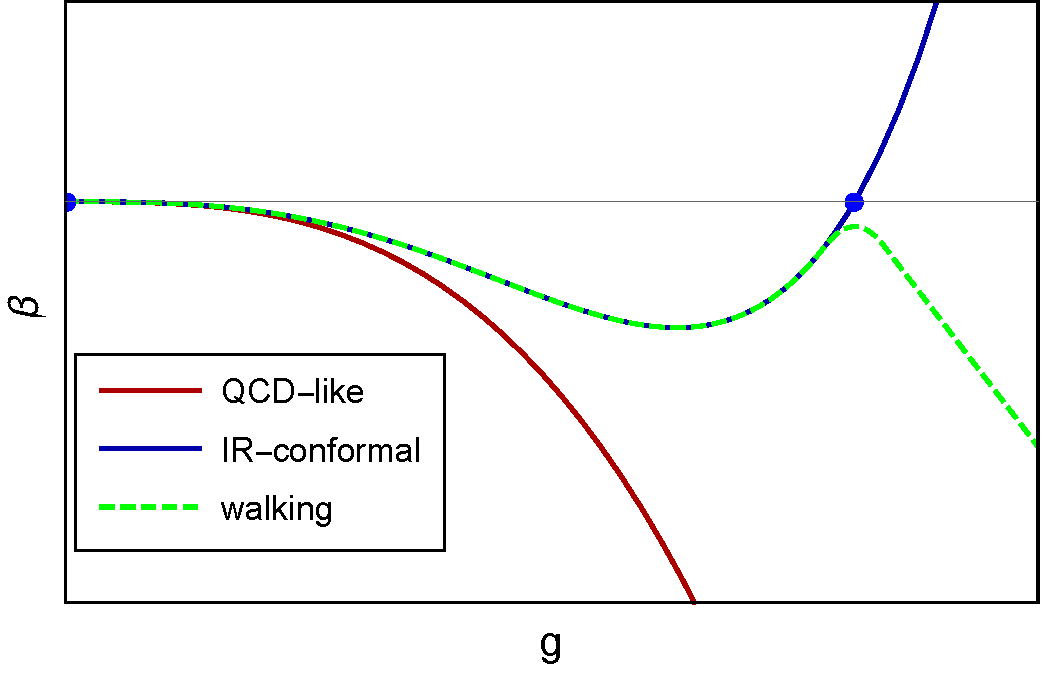
\includegraphics[width=0.5\textwidth]{pics/beta_walking}~~~
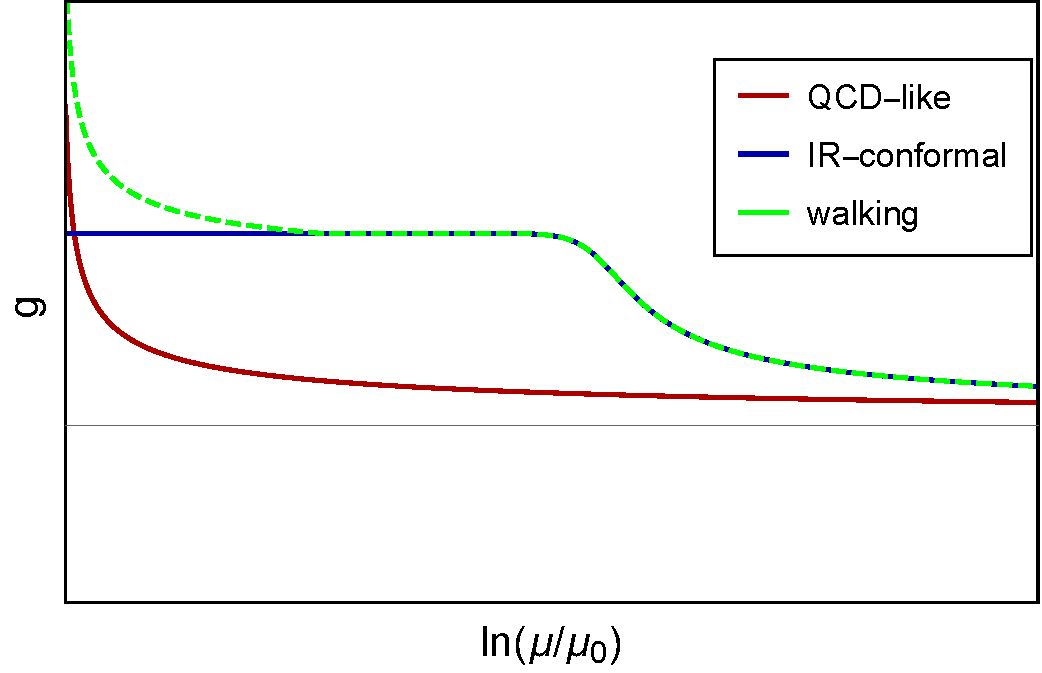
\includegraphics[width=0.5\textwidth]{pics/g_walking}
\caption{Beta function (left panel) and gauge coupling (right panel) for three different kinds of theories: a QCD-like theory (red line), a theory in the conformal window (blue line) and a theory with walking gauge coupling (green dashed line). In the right panel, the gauge coupling is plotted as a function of the energy scale $\mu$ over some reference scale $\mu_0$.} 
\label{walking}
\end{figure}


%REMEMBER TO JUSTIFY THE FACT THAT THE NUMBER OF FLAVOURS IS TREATED LIKE A CONTINUOUS PARAMETER!

%%%%%%%%%%%%%%%%%%%%%%%%%%%%%%%%%%%%%%%%%%%%%%%%%%%%%%

\section{Transport coefficients}


%%%%%%%%%%%%%%%%%%%%%%%%%%%%%%%%%%%%%%%%%%%%%%%%%%%%%%

\section{Transport coefficients of a gauge theory: the kinetic approach}


%%%%%%%%%%%%%%%%%%%%%%%%%%%%%%%%%%%%%%%%%%%%%%%%%%%%%%

\section{Application to theories in the conformal window}

%%%%%%%%%%%%%%%%%%%%%%%%%%%%%%%%%%%%%%%%%%%%%%%%%%%%%%
